\section{图表示例}
由于该模板服务于湖南大学机械与运载工程学院于2025年末发布的新的本科生毕业论文撰写规范（适用于2026年毕业生），为了实现撰写规范中的一些要求，新定义了一些命令。在此处将这些命令和一些其他常用的命令进行一些演示和说明。

首先是表注：
\begin{table}[ht]
    \abovetopsep=0pt
    \aboverulesep=0pt
    \belowrulesep=0pt
    \belowbottomsep=0pt
    \begingroup
    \centering
    \caption{获奖}
    \label{tab:table1}
    \fontSimsun\sizeFive
    \newcolumntype{Z}{>{\centering\arraybackslash}X}
    \begin{tabularx}{\textwidth}{Z|Z|Z|Z}
        \toprule
        年份                    & 奖项                                              & 类别         & 结果 \\
        \hline
        2022                  & 金摇杆奖                                            & 最受期待游戏     & 提名 \\
        \hline
        \multirow{6}{*}{2023} & 2023世界科幻游戏年度大奖                                  & 最佳人气奖      & 获奖 \\
        \cline{2-4}
        & \multirow{3}{0.25\textwidth}{Google Play年度最佳榜单} & 最佳游戏       & 获奖 \\
        \cline{3-4}
        &                                                 & 最佳剧情游戏     & 获奖 \\
        \cline{3-4}
        &                                                 & 最佳平板游戏     & 获奖 \\
        \cline{2-4}
        & App Store Awards                                & 年度iPhone游戏 & 获奖 \\
        \cline{2-4}
        & 2023年游戏大奖                                       & 最佳手机游戏     & 获奖 \\
        \bottomrule
    \end{tabularx}
    \endgroup

    \vspace{3pt}
    \fontSimsun\sizeFivel 注：仅供参考。
    \vspace{-15pt}
\end{table}

本来定义了表注的命令tablenotes，但是有一些bug，修复半天修复不了，懒得搞了，所以直接定义字体和大小吧。

然后是三线表：
\begin{table}[htbp]
    \abovetopsep=0pt
    \aboverulesep=0pt
    \belowrulesep=0pt
    \belowbottomsep=0pt
	\centering
	\begin{threeparttable}[c]
		\caption{三线表}
		\label{tab:ch1-part-rotate}
		\tableBodyFont
        \begin{tabular}{lcc}
			\toprule
			换热器  & 热边压降损失    & 冷边压降损失               \\
			\midrule
			初级&2974.37&2931.52\\
			次级&2924.65&3789.76\\
			\bottomrule  
		\end{tabular}
	\end{threeparttable}
\end{table}

其次是行内文献引用：

“设定L3下表面固定，上表面施加0.2 MPa的均匀压力载荷，计算其轴向压缩响应。计算得出单椎体轴向等效刚度约为8200 N/mm，符合健康年轻男性裸椎的高刚度特征。通过与文献\inlinecite{nekkanty2010stiffness}中对尸体进行的实验数据的比对，验证了本文逆向建模边界的准确性与材料参数设置的合理性。此步骤确立了基准模型，可进一步开展后续的双节段系统仿真。”

接下来是分图排版：
\begin{figure}[H]
    \centering
    \begin{subfigure}[b]{0.3\textwidth}
        \centering
        \includegraphics[width=\textwidth]{example-image-a}
        \caption{分图A} 
    \end{subfigure}
    \hfill
    \begin{subfigure}[b]{0.3\textwidth}
        \centering
        \includegraphics[width=\textwidth]{example-image-b}
        \caption{分图B} 
    \end{subfigure}
    \caption{总图名}
\end{figure}

第二类分图排版：
\begin{figure}[H]
    \centering
    \subfloat[这是啥]{\label{1} 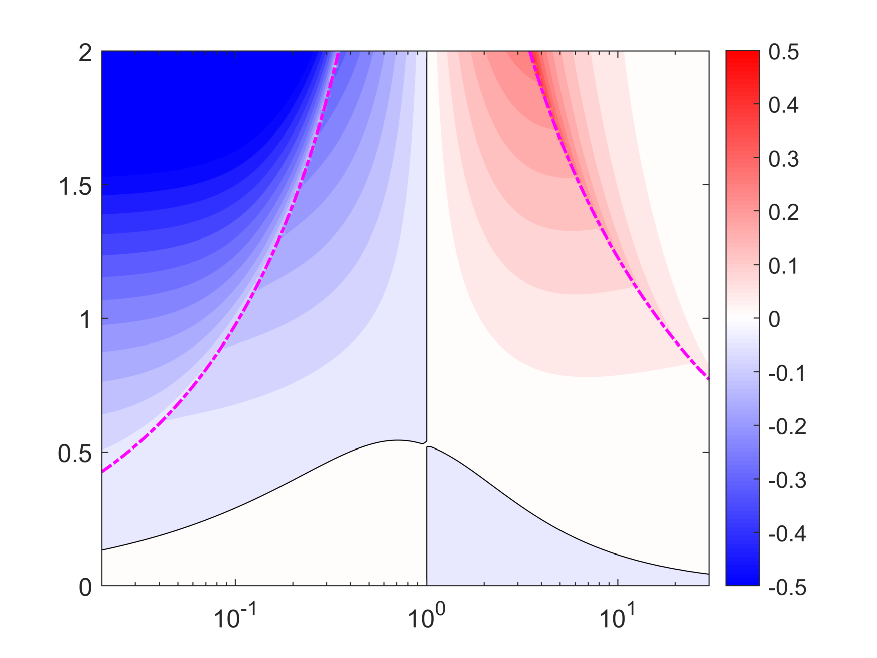
\includegraphics[width=0.5\linewidth]{docs/imgs/overpic_example}}
    \subfloat[这又是啥]{\label{2} 
\includegraphics[width=0.35\linewidth]{docs/imgs/HSR}}
    \caption{分图2}
    \label{不知道是啥}
\end{figure}

图注：
\begin{figure}[H]
    \centering
    
\includegraphics[width=100pt]{docs/imgs/herta}
    \figurenotes{这是图注或其他说明。} 
    \caption{签名}
    \label{fig:figure2}
\end{figure}

最后是有序列表：
\begin{enumerate}
    \item \textbf{有序列表1}：有序列表1有序列表1有序列表1有序列表1有序列表1有序列表1有序列表1有序列表1有序列表1有序列表1有序列表1有序列表1有序列表1有序列表1有序列表1有序列表1
    \item \textbf{有序列表2}：有序列表2有序列表2有序列表2有序列表2有序列表2有序列表2有序列表2有序列表2有序列表2有序列表2有序列表2
    \item \textbf{有序列表3}：有序列表3有序列表3有序列表3有序列表3
\end{enumerate}

和无序列表：
\begin{itemize}
    \item \textbf{无序列表1}：无序列表1无序列表1无序列表1无序列表1无序列表1无序列表1无序列表1
    \item \textbf{无序列表2}：无序列表2无序列表2无序列表2无序列表2无序列表2无序列表2无序列表2无序列表2
    \item \textbf{无序列表3}：无序列表3无序列表3无序列表3无序列表3无序列表3
\end{itemize}

其他请自行学习\LaTeX{}。因为\LaTeX{}是世界上最好的语言（误）！推荐阅读：董晟渤\footnote{北京大学，数学科学学院，概率论与数理统计在读博士}的博客内容：《LaTeX：从入门到日常使用》https://dylandong.top/posts/e480。
